\chapter{Formas e sólidos}\label{ch:g2:shapes}

As formas planas vivem no papel; os sólidos enchem as suas mãos.
Este capítulo classifica as formas planas contando lados e cantos,
testa o ângulo reto com um canto de papel dobrado e apresenta os
primeiros sólidos --- cujas \omterm{def:g2:shapes:solids}{faces} são as formas planas que já
conhecemos.

\section{Classificar as formas planas}

\begin{definition}[De lados retos e redondas]\label{def:g2:shapes:sort}
Uma forma cujo contorno é feito só de lados retos é um
\emph{polígono}\index{polígono}: triângulo ($3$ lados), quadrilátero ($4$ lados:
quadrados e retângulos são quadriláteros), pentágono ($5$),
hexágono ($6$). Uma forma de contorno curvo, como o círculo,
\emph{não} é um polígono.
\end{definition}

\begin{omfigure}
\begin{tikzpicture}[scale=0.62]
  \draw[thick, fill=omDef!12] (0,0) -- (1.8,0) -- (0.9,1.5) -- cycle;
  \node[below, font=\small] at (0.9,-0.35) {$3$ lados};
  \begin{scope}[xshift=3.2cm]
  \draw[thick, fill=omThm!12] (0,0) rectangle (1.7,1.5);
  \node[below, font=\small] at (0.85,-0.35) {$4$ lados};
  \end{scope}
  \begin{scope}[xshift=6.6cm]
  % pentagono dimensionado para ocupar a mesma faixa de altura dos vizinhos
  \draw[thick, fill=omMeth!12] (0.95,0.67) +(90:0.83) -- +(162:0.83) --
    +(234:0.83) -- +(306:0.83) -- +(18:0.83) -- cycle;
  \node[below, font=\small] at (0.95,-0.35) {$5$ lados};
  \end{scope}
  \begin{scope}[xshift=10.0cm]
  \draw[thick, fill=omProp!12] (0.75,0.75) circle (0.75);
  \node[below, font=\small] at (0.75,-0.35) {redonda};
  \end{scope}
\end{tikzpicture}

{\small Classificação pelo número de lados. O número de cantos é
sempre igual ao número de lados.}
\end{omfigure}

\begin{method}[Testar um ângulo reto]\label{met:g2:shapes:rightangle}
Dobre uma folha de papel duas vezes para formar um canto bem
definido --- esse canto é um ângulo reto. Encaixe-o no canto de uma
forma:
\begin{enumerate}
  \item se os dois lados da forma correrem exatamente ao longo do
        canto dobrado, o ângulo é reto;
  \item se o canto for mais aberto ou mais fechado, não é reto.
\end{enumerate}
Um quadrado e um retângulo têm quatro ângulos retos.
\end{method}

\section{Reproduzir na malha quadriculada}

\begin{method}[Copiar uma figura]\label{met:g2:shapes:copy}
No papel quadriculado, copie uma figura vértice por vértice:
\begin{enumerate}
  \item escolha um canto e marque-o na malha vazia;
  \item conte os quadradinhos até o canto seguinte (``$3$ para a
        direita, $2$ para cima'') e marque-o;
  \item ligue os cantos em ordem e compare com o modelo.
\end{enumerate}
\end{method}

\begin{omfigure}
\begin{tikzpicture}[scale=0.5]
  \draw[gray!40] (0,0) grid (5,4);
  \draw[thick, omDef] (1,1) -- (4,1) -- (4,3) -- (2,3) -- cycle;
  \begin{scope}[xshift=7cm]
  \draw[gray!40] (0,0) grid (5,4);
  \draw[thick, omThm] (1,1) -- (4,1) -- (4,3) -- (2,3) -- cycle;
  \node[font=\footnotesize, omThm, below] at (2.5,-0.15) {a cópia};
  \end{scope}
\end{tikzpicture}

{\small Uma figura e a sua cópia, feita contando os quadradinhos
entre os cantos.}
\end{omfigure}

\section{Sólidos}

\begin{definition}[Os primeiros sólidos]\label{def:g2:shapes:solids}
Os sólidos ocupam espaço. Os seus lados planos são as
\emph{faces}\index{face}:
\begin{itemize}
  \item o \emph{cubo}\index{cubo}: $6$ faces quadradas (um dado);
  \item o \emph{bloco retangular} (prisma de base retangular): $6$
        faces retangulares (uma caixa de cereal);
  \item o \emph{cilindro}\index{cilindro}: duas faces redondas e uma lateral
        enrolada (uma lata);
  \item a \emph{bola}: perfeitamente redonda, sem face plana.
\end{itemize}
Os sólidos e as suas faces voltam no \cref{ch:g5:solids}.
\end{definition}

\begin{omfigure}
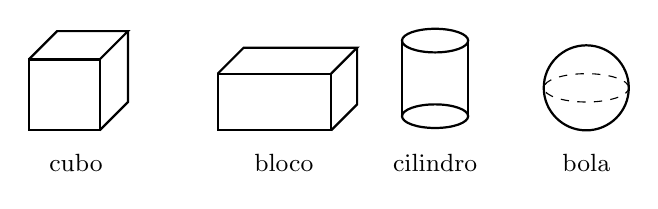
\begin{tikzpicture}[scale=0.6]
  \draw[thick] (0,0) rectangle (1.5,1.5);
  \draw[thick] (0,1.5) -- (0.6,2.1) -- (2.1,2.1) -- (1.5,1.5);
  \draw[thick] (2.1,2.1) -- (2.1,0.6) -- (1.5,0);
  \node[below, font=\small] at (1.0,-0.3) {cubo};
  \begin{scope}[xshift=4.0cm]
  \draw[thick] (0,0) rectangle (2.4,1.2);
  \draw[thick] (0,1.2) -- (0.55,1.75) -- (2.95,1.75) -- (2.4,1.2);
  \draw[thick] (2.95,1.75) -- (2.95,0.55) -- (2.4,0);
  \node[below, font=\small] at (1.4,-0.3) {bloco};
  \end{scope}
  \begin{scope}[xshift=8.6cm]
  \draw[thick] (0,0.3) ellipse (0.7 and 0.25);
  \draw[thick] (-0.7,0.3) -- (-0.7,1.9);
  \draw[thick] (0.7,0.3) -- (0.7,1.9);
  \draw[thick] (0,1.9) ellipse (0.7 and 0.25);
  \node[below, font=\small] at (0,-0.3) {cilindro};
  \end{scope}
  \begin{scope}[xshift=11.8cm]
  \draw[thick] (0,0.9) circle (0.9);
  \draw[dashed] (0,0.9) ellipse (0.9 and 0.3);
  \node[below, font=\small] at (0,-0.3) {bola};
  \end{scope}
\end{tikzpicture}

{\small Os primeiros sólidos. Passe o dedo por um \omterm{def:g2:shapes:solids}{cubo}: você sente
$6$ \omterm{def:g2:shapes:solids}{faces} planas e arestas vivas; a bola não tem nenhuma.}
\end{omfigure}

\section{Exercícios}

\begin{exercise}[$\star$]\label{exo:g2:shapes:1}
Para cada uma, conte lados e cantos e dê o nome: uma forma com $5$
lados; uma forma com $3$ cantos; uma forma redonda.
\end{exercise}

\begin{exercise}[$\star$]\label{exo:g2:shapes:2}
Separe em ``\omterm{def:g2:shapes:sort}{polígono}'' e ``não é \omterm{def:g2:shapes:sort}{polígono}'': um quadrado; um
círculo; um triângulo; um hexágono.
\end{exercise}

\begin{exercise}[$\star$]\label{exo:g2:shapes:3}
Faça um testador de ângulo reto dobrando papel. Encontre três
ângulos retos na sala e um ângulo que não seja reto.
\end{exercise}

\begin{exercise}[$\star$]\label{exo:g2:shapes:4}
Quantos ângulos retos tem um quadrado? E um retângulo? E, no máximo,
quantos pode ter um triângulo? (Tente desenhar um com dois.)
\end{exercise}

\begin{exercise}[$\star$]\label{exo:g2:shapes:5}
No papel quadriculado, copie um retângulo de $4$ quadradinhos de
largura por $2$ de altura e depois um triângulo com base de $3$
quadradinhos.
\end{exercise}

\begin{exercise}[$\star$]\label{exo:g2:shapes:6}
Dê o nome do sólido: um dado; uma lata de sopa; uma bola de futebol;
uma caixa de sapatos.
\end{exercise}

\begin{exercise}[$\star$]\label{exo:g2:shapes:7}
Quantas \omterm{def:g2:shapes:solids}{faces} tem um \omterm{def:g2:shapes:solids}{cubo}? Que forma tem cada \omterm{def:g2:shapes:solids}{face}? E quantas \omterm{def:g2:shapes:solids}{faces}
tem um bloco retangular?
\end{exercise}

\begin{exercise}[$\star$]\label{exo:g2:shapes:8}
Quais sólidos rolam: o \omterm{def:g2:shapes:solids}{cubo}, o bloco retangular, a bola, o \omterm{def:g2:shapes:solids}{cilindro}?
Por quê?
\end{exercise}

\begin{exercise}[$\star$]\label{exo:g2:shapes:9}
Uma forma tem $6$ lados. Como ela se chama? Quantos cantos tem?
\end{exercise}

\begin{exercise}[$\star\star$]\label{exo:g2:shapes:10}
No papel quadriculado, desenhe uma casa: um quadrado para a parede
($4 \times 4$) com um telhado triangular em cima. Quantos lados e
quantos cantos tem o contorno inteiro da casa?
\end{exercise}
